\chapter{实验与分析}
\section{实验结果}
\subsection{实验设置以及测试方法}
我们的网络实现是基于Pytorch的,pytorch是主要基于python的深度学习框架,其承担着很多深度学习模型在算法层面上最底层的设计和实现。其作为一个动态的建图工具,能将tensor放到GPU上进行运算加速,有很好的灵活性。

pytorch是基于Cpython的API进行设计的,对于Python有着良好的支持,能够较为容易地进行调试和运行,又由于其对于动态图的支持和类似底层的实现,pytorch有着优秀的运行速度和灵活性。

由于我们使用的数据集dagm是图像,且其标注并非使用的标准格式,我们在cornernet的基础上实现了数据的转换和标注的自动生成,并重构了网络的输入接口,通过C代码对标注的访问和生成实现加速。

dagm数据集有8000张缺陷图片,我们的训练平台基于Nvidia GTX1070,驱动版本418.56,CUDA版本10.1。没有使用分布式训练。

\subsection{模型的训练}
我们创建了基于第四章的网络结构的Pytorch网络,在Hourglass模块、残差模块的基础上引申出了我们的CornerNet网络,构建了fire module、分离了其中的各通道,进行训练。

模型训练参数被提前放到config下的对应网络名字的文件中,并在一定次数的循环之后,保存网络的当时各参数到缓存中。

我们使用的是基于三个损失函数的参数训练方法,并设置有学习率的自动下降。

\subsection{实验结果}

我们运行了我们的网络,并预测了缺陷所在位置,我们将其标记了出来,如下图\ref{fig:dagm-after}所示。

\begin{figure}[!tbp]
    \centering
    \begin{minipage}[b]{0.4\textwidth}
      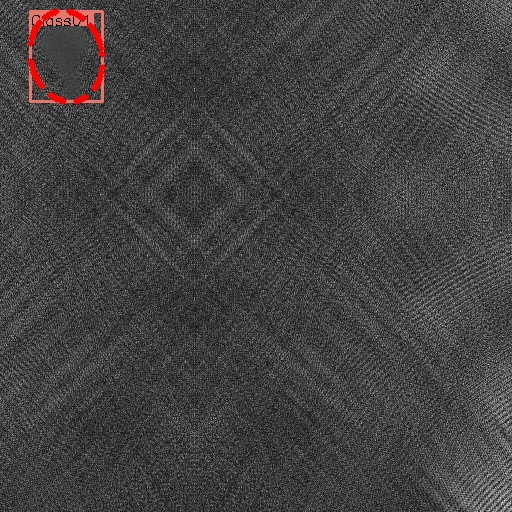
\includegraphics[width=\textwidth]{figures/33-0.jpg}
    \end{minipage}
    \hfill
    \begin{minipage}[b]{0.4\textwidth}
      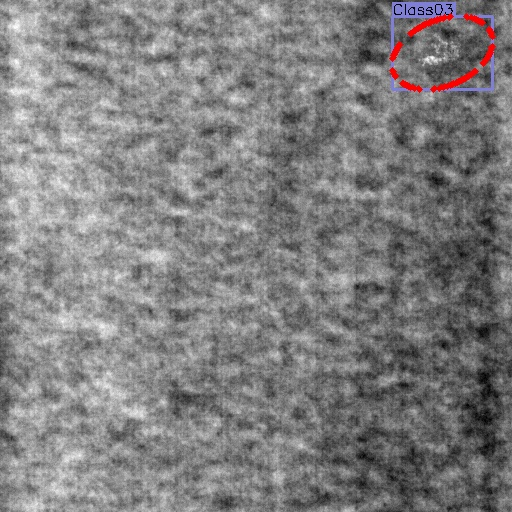
\includegraphics[width=\textwidth]{figures/167-0.jpg}
    \end{minipage}
    \caption{处理后的dagm的原图标注}
    \vspace{-1em}
\end{figure}


\begin{figure}[!tbp]
    \centering
    \begin{minipage}[b]{0.4\textwidth}
      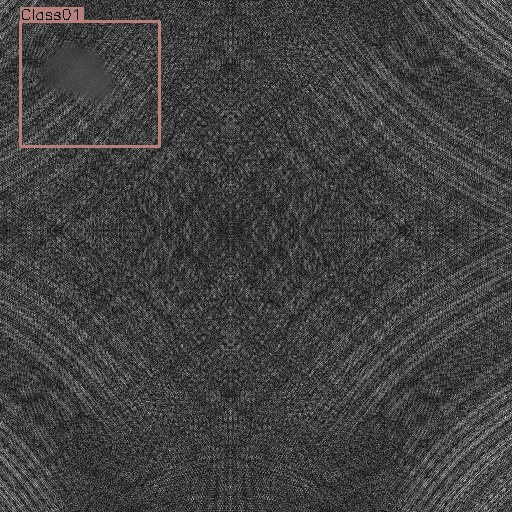
\includegraphics[width=\textwidth]{figures/33.jpg}
    \end{minipage}
    \hfill
    \begin{minipage}[b]{0.4\textwidth}
      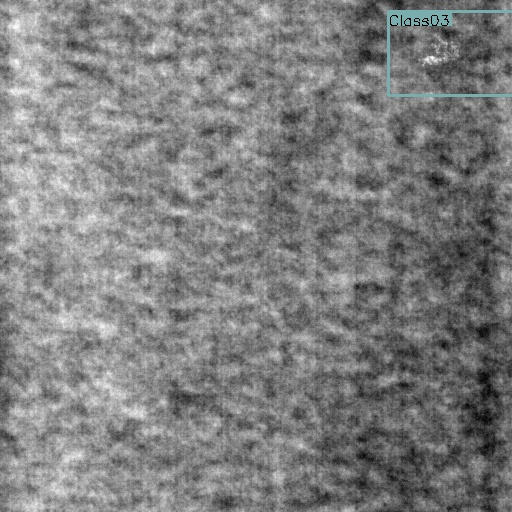
\includegraphics[width=\textwidth]{figures/167.jpg}
    \end{minipage}
    \caption{dagm图片的预测框}
    \label{fig:dagm-after}
    \vspace{-1em}
\end{figure}

此外我们对我们的数据集进行了评价,如下表\ref{table:result}:

\begin{table}[htbp]
	\caption{CornerNet和centerNet在dagm数据集上的AP比较}\label{table:result}
  \vspace{0.5em}\centering\wuhao
  \resizebox{\textwidth}{18mm}{
    \begin{tabular}{c|ccc|cccccc}
      \toprule[1.5pt]
      Method & Backbone & Train input & Test input & AP & $ AP_{50} $ & $ AP_{75} $ & $ AP_{S} $ & $ AP_{M} $ & $ AP_{L} $\\
      \midrule[1pt]
          CornerNet-511 & Hourglass-104 & 512 $ \times $ 512 & ori. & 0.331 & 0.655 & 0.287 & 0.331 & 0.398 & 0.277 \\
          CornerNet\_Saccade-511 & Hourglass-104 & 512 $ \times $ 512 & ori. & 0.448 & 0.844 & 0.408 & 0.251 & 0.444 & 0.494 \\ 
          CornerNet\_Squeeze-511 & Hourglass-104 & 512 $ \times $ 512 & ori. & 0.541 & 0.888 & 0.595 & 0.445 & 0.579 & 0.537 \\ 
          CenterNet-52 & Hourglass-52 & 512 $ \times $ 512 & ori. & 0.494 & 0.875 & 0.506 & 0.448 & 0.563 & 0.453 \\
      \bottomrule[1.5pt]
    \end{tabular}
  }
	\vspace{\baselineskip}
\end{table}



\begin{table}[htbp]
	\caption{CornerNet和centerNet在dagm数据集上的AR比较}\label{table}
  \vspace{0.5em}\centering\wuhao
  \resizebox{\textwidth}{18mm}{
    \begin{tabular}{c|ccc|cccccc}
      \toprule[1.5pt]
      Method & Backbone & Train input & Test input & $ AR_{1} $ & $ AR_{10} $ & $ AR_{100} $ & $ AR_{S} $ & $ AR_{M} $ & $ AR_{L} $ \\
      \midrule[1pt]
          CornerNet-511 & Hourglass-104 & 512 $ \times $ 512 & ori. & 0.415 & 0.452 & 0.482 & 0.421 & 0.533 & 0.410 \\
          CornerNet\_Saccade-511 & Hourglass-104 & 512 $ \times $ 512 & ori. & 0.503 & 0.625 & 0.635 & 0.320 & 0.623 & 0.698 \\ 
          CornerNet\_Squeeze-511 & Hourglass-104 & 512 $ \times $ 512 & ori. & 0.541 & 0.888 & 0.595 & 0.445 & 0.579 & 0.537 \\
          CenterNet-52 & Hourglass-52 & 512 $ \times $ 512 & ori. & 0.536 & 0.619 & 0.645 & 0.517 & 0.673 & 0.608\\
      \bottomrule[1.5pt]
    \end{tabular}
  }  
	\vspace{\baselineskip}
\end{table}

\section{优化方法}
网络训练优化是网络性能的重要方面,为此我们需要优化我们的训练步骤:

\begin{enumerate}
    \item 数据增强:因为我们的数据集有效缺陷样本并不多,我们需要更多的数据源,图像增强是我们的一个很好的方法,通过对原图的旋转、翻转、切割、放缩和添加噪声等处理,能够增加网络处理的泛化能力,实现更高的网络识别性能。
    \item 预处理:预处理中比如归一化能够让不同维度的数据具有相同的分布,让梯度的优化能够尽量使用接近的迭代方案。
    \item 参数初始化:初始参数的选择是网络最终性能的一个很好的保证,如果初始参数偏差过大,很可能到最后由于梯度陷阱问题而无法得到真实参数。随机数和合适的分布是极其重要的。
    \item 网络参数:如卷积核的选取应该尽量小用以节省计算资源,提升速度。学习率的选取和自调整是训练损失函数的重要参数。
    \item 预训练:现在有很多模型,且之前对于这些的研究有很多成果,使用这些以前已经训练过的模型能够让网络更快地进行泛化,在顶层的通用性可以让模型忽视底层模型的不同。
\end{enumerate}

\section{本章总结}

本章是我们探究了我们模型的实现和训练方法,并叙述了我们方案的最终实现结果。并将其和以前的相关成果进行了比较和分析,能够发现我们的模型在时间和精度上均有较好的表现。此外我们还探究了模型的训练和优化方案,提出了我们应该如何对我们的模型进行改进。